\chapter{Introdução} \label{cap:introducao}
\setcounter{table}{0}
    A ideia de um robô solucionador de labirintos surge da década de 50 do século passado e foi concebido já como um robô autônomo, isto é, sem interferência humana no processo de pilotagem. 
    
    As competições de robôs capazes de resolver labirintos, popularmente chamados de \textit{micromouse}, por sua vez, datam da década de 70, quando foram lançados como competição do \gls{IEEE}, conforme mostrado em \citeonline{day1979amazing}. Estas competições até hoje são muito populares na Europa. Em países como o Reino Unido se destaca a \textit{UK micromouse}, em Portugal a \textit{Micromouse Portuguese Contest} e no Japão a \textit{all japan micromouse robot competition}. Este último é referência mundial nesse quesito e seus competidores são referências pelas mais diversas tecnologias empregadas, diferentes técnicas de aperfeiçoamento e diminutos tempos com que conseguem resolver e percorrer complexos labirintos \cite{borges2013micromouse}.

    A competição, resumidamente, consiste em resolver um labirinto, dividido em células, até encontrar o seu centro, partindo de um dos seus cantos, no menor tempo possível e, sempre, de forma autônoma, ou seja, os projetistas não podem operar o robô durante o percurso. 
    
    A seguir são listadas exemplos de regras para o caso japonês, conforme encontrado em \citeonline{micromouse-rules-japan-2023}.

    \begin{itemize}
        \item O \textit{Micromouse} deve ser autossuficiente. Não é permitida a utilização de fontes de energia baseadas em combustão.
        \item Nenhum componente de hardware ou software do \textit{Micromouse} pode ser adicionado, removido, substituído ou modificado pelo operador durante a competição. Entretanto, pequenos reparos e ajustes são permitidos.
        \item O \textit{Micromouse} não deve saltar, escalar, danificar ou romper as paredes do labirinto.
        \item O labirinto deve ser composto por células unitárias de $9\,\text{cm} \times 9\,\text{cm}$, sendo que seu tamanho total não pode exceder $32 \times 32$ células. A altura das paredes de cada célula deve ser de $2,5\,\text{cm}$ e sua espessura de $0,6\,\text{cm}$ (Figura \ref{fig:celulas-labirinto}).
        \item O ponto de partida do labirinto localiza-se em um dos quatro cantos, sendo a orientação inicial definida no sentido horário. O ponto de chegada consiste em uma área retangular previamente determinada (Figura \ref{fig:labirinto-micromouse-japao}).
        \item Não é permitido ao operador inserir qualquer informação sobre o labirinto no \textit{Micromouse} após a divulgação do percurso.
        \item Considera-se que um \textit{Micromouse} concluiu o labirinto quando todas as partes de sua estrutura estiverem completamente inseridas na área de chegada. 
    \end{itemize}

    \begin{figure}[htb]
        \centering
        \Caption{\label{fig:celulas-labirinto} Formato da célula do labirinto}
        \UFCfig{}{
            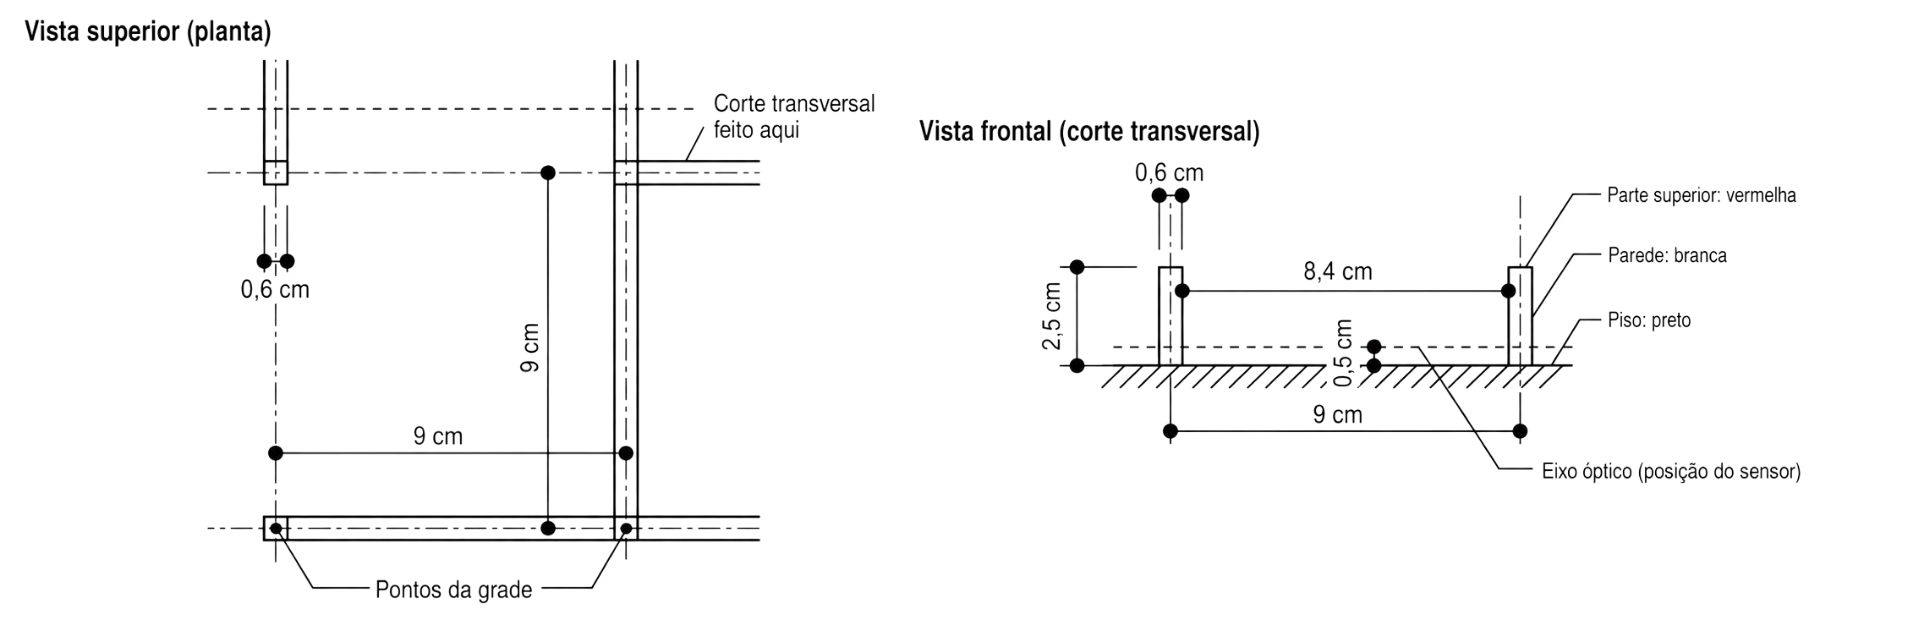
\includegraphics[width=12cm]{figuras/introducao/celula-labirinto-japao.png}
        }{
            \Fonte{Adaptado de \citeonline{micromouse-rules-japan-2023}}
        }	
    \end{figure}

    \begin{figure}[htb]
        \centering
        \Caption{\label{fig:labirinto-micromouse-japao} Labirinto do \textit{All Japan Micromouse Robot Competition}}
        \UFCfig{}{
            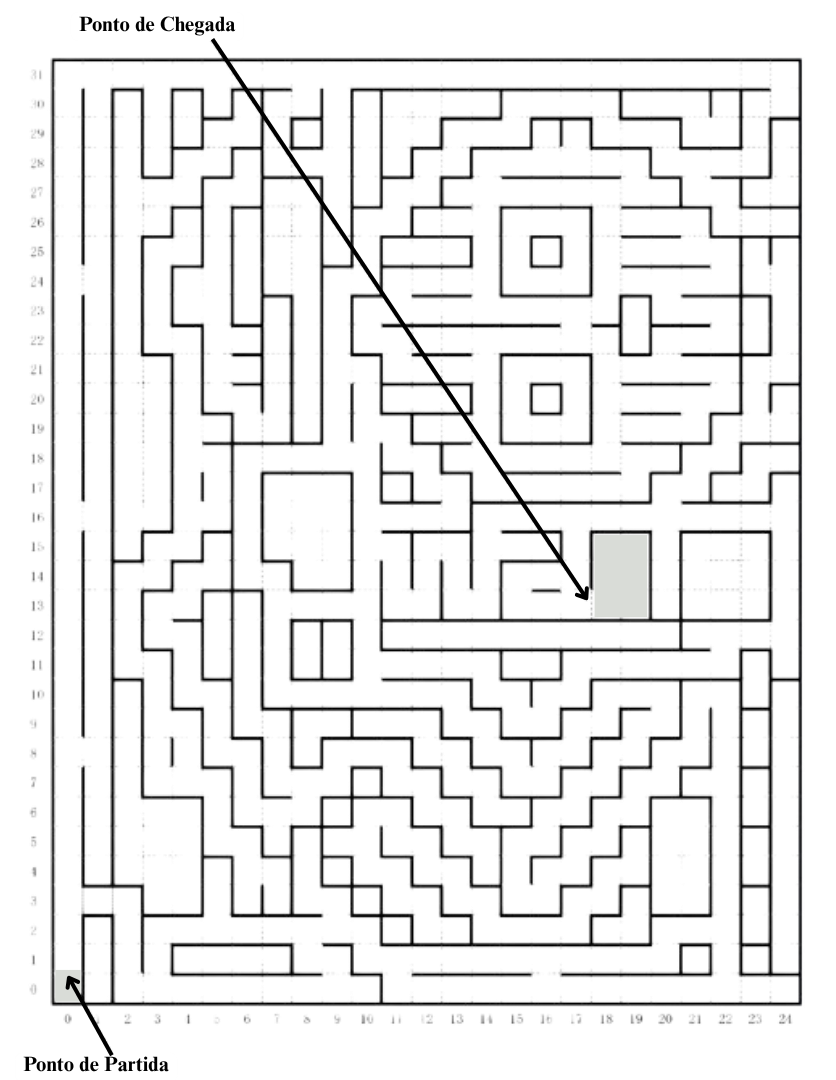
\includegraphics[width=7cm]{figuras/introducao/labirinto-japao.png}
        }{
            \Fonte{Adaptado de \citeonline{micromouse-rules-japan-2023}}
        }	
    \end{figure}

    Por já estar consolidado como um desafio dentro das engenharias, diversas abordagens são feitas ao redor do tópico do robô \textit{micromouse}. 
    
    Em \citeonline{su-et-al-2013} faz-se a implementação de uma versão simulada do comportamento do robô nos ambientes MATLAB/SIMULINK a fim de analisar questões relativas à resolução de labirinto, planejamento de trajetória e, também, técnicas de controle no contexto da cinemática diferencial do \textit{micromouse}.

    Já em \citeonline{micromouse-kit-educational} trabalha-se a implementação prática do robô a partir de um kit educacional desenvolvido em contexto escolar a fim de baratear os custor de uso quando comparados aos robôs comerciais. O referido kit conta com um microcontrolador dsPIC30F6010 e sua comunicação ocorre via porta serial com RS232. A Figura \ref{fig:kit} apresenta o robô utilizado pelos autores.

    \begin{figure}[htb]
        \centering
        \Caption{\label{fig:kit} Kit utilizado pelos autores}
        \UFCfig{}{
            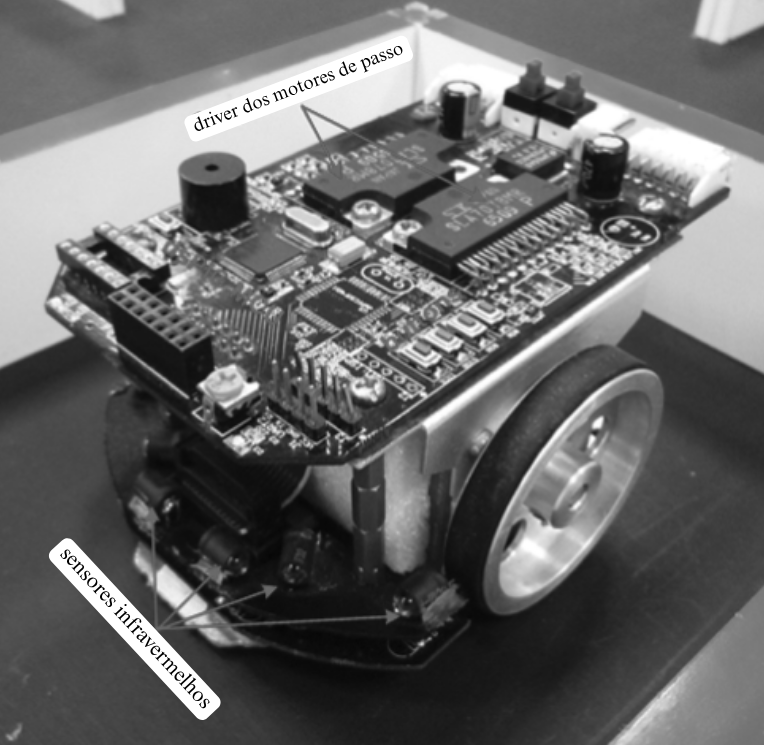
\includegraphics[width=7cm]{figuras/introducao/kit-micromouse-su-et-al.png}
        }{
            \Fonte{Adaptado de \citeonline{micromouse-kit-educational}}
        }	
    \end{figure}

    Em cenário nacional, é possível considerar ainda o trabalho de \citeonline{roberto-et-al-2024}, os quais desenvolvem um robô \textit{micromouse} desde o começo apresentando todos os seus aspectos construtivos e desenvolvendo as diversas malhas de controle para os cenários de resolução de labirinto. É cabível citar também o trabalho de \citeonline{dissetacao-pereira-2000}, o qual -- apesar de não abordar diretamente sobre resolução de labirintos -- desenvolve análises importantes dos aspectos cinemáticos, dinâmicos e dentro da teoria de controle, que podem ser aplicados para a implementação de robôs móveis e com restrições de movimento.

    \section{Motivação} \label{sec:motivacao}

        O desenvolvimento de um \textit{micromouse}, caracteriza-se por seu caráter multidisciplinar, uma vez que integra conhecimentos advindos de outras áreas da Engenharia. A concepção desse tipo de sistema demanda competências relacionadas ao desenvolvimento de eletrônica embarcada, técnicas de programação (muitas vezes envolvendo linguagens de alto e baixo nível simultaneamente), teoria de Controle, implementação de algoritmos inteligentes, projeto de placas de circuito impresso, modelagem mecânica do movimento, conhecimento de micromotores elétricos, integração de sensores, sistemas de comunicação sem fio, entre outras tecnologias essenciais para a operação autônoma do robô \cite{kim-byung-2020}.

        % Dos pontos enumerados anteriormente, alguns podem ser contornados total ou parcialmente com a adoção de modelos já prontos como, por exemplo, o kit educacional em \citeonline{micromouse-kit-educational} ou, para o caso do presente trabalho o kit desenvolvido em \citeonline{manual-microumouse-2015}.

        Parte desses desafios pode ser reduzida por meio da utilização de plataformas já consolidadas. Como exemplos, podem ser citados o kit educacional apresentado em \citeonline{micromouse-kit-educational} e, no contexto deste trabalho, a plataforma descrita em \citeonline{manual-microumouse-2015}, a qual serviu de base para o desenvolvimento realizado.

        % Entretanto, os tópicos relativos à programação, à modelagem e ao controle não são contornados dessa forma, haja vista que a forma com que são construídos, visando trabalhar em diferentes situações e ambientes, faz com que essas questões devam ser adaptadas a cada realidade.

        Entretanto, os aspectos relacionados à programação, à modelagem e ao controle do sistema permanecem fortemente dependentes da aplicação considerada. Embora modelos previamente desenvolvidos forneçam uma estrutura funcional para o robô, os algoritmos de controle e navegação devem ser adequadamente adaptados às características da plataforma utilizada e às condições específicas do ambiente de operação.

        % Portanto, neste cenário, este trabalho se motiva pelo estudo do controle aplicado ao robô \textit{micromouse} disponível no laboratório da \gls{UFPI} através do grupo \gls{GRASI}. Para isso é feita uma análise da cinemática/dinâmica do robô e do comportamento dos seus motores com sinais de excitação, especialmente para a resposta ao degrau unitário na presença de sinais \gls{PRBS}. Conjuntamente, são projetados controladores monovariáveis para atuar nas dinâmicas individuais dos motores e na dinâmica global do robô. Por fim, são desenvolvidos algorítmos \textit{seguidores de parede} os quais são a base para algumas das técnicas de resolução de labirintos. 

        Nesse contexto, este trabalho tem como motivação o estudo e o desenvolvimento de estratégias de controle aplicadas ao robô \textit{micromouse} disponível no Laboratório de Controle e Automação do curso de Engenharia Elétrica da \gls{UFPI}, por meio das atividades desenvolvidas no âmbito do grupo \gls{GRASI}. Para isso, é realizada uma análise da cinemática e da dinâmica do robô, bem como do comportamento dinâmico de seus motores diante de diferentes sinais de excitação, com ênfase na resposta ao degrau e na utilização de sinais \gls{PRBS} para fins de identificação e caracterização do sistema.

        De posse dos modelos obtidos, são projetados controladores monovariáveis destinados ao controle das dinâmicas individuais dos motores e das variáveis globais de movimento do robô. Adicionalmente, são desenvolvidos algoritmos do tipo \textit{seguidor de parede}, amplamente empregados em estratégias de navegação e considerados a base para diversos métodos clássicos de resolução de labirintos utilizados em competições de \textit{micromouse}.

    % objetivos
    \section{Objetivos} \label{sec:objetivos}

        \subsection{Objetivo Geral} \label{ssec:objetivo-geral}

        Desenvolver e implementar estratégias de controle de velocidade e telemetria para um robô autônomo do tipo \textit{micromouse}, visando melhorar seu desempenho de navegação e movimentação.

        \subsection{Objetivos Específicos} \label{ssec:objetivos-especificos}

        \begin{itemize}
            \item Identificar e modelar o comportamento dos motores através da descrição no tempo, \gls{FT} e equações a diferenças.
            \item Estudar o comportamento diferencial do robô \textit{micromouse} por meio de equações cinemáticas.
            \item Projetar, implementar e avaliar controladores básicos do tipo \gls{PID} para os motores e para as velocidades globais do robô, com o uso de malhas de controle e de supervisão.
            \item Desenvolver estratégias de comunicação sem fio que permitam a telemetria e a adequada coleta de informações do robô \textit{micromouse} mesmo quando não estiver fisicamente próximo ao \gls{PC}.
            \item Desenvolver algorítmos em linguagem de programação \textit{C} que possam ser aplicadas a sistemas embarcados a partir da adapatação de algoritmos desenvolvidos em linguagem \textit{MATLAB}.
        \end{itemize}

    % seções 
    \section{Organização do Trabalho} \label{sec:organização}

        O presente trabalho está dividido em cinco capítulos. No Capítulo \ref{cap:id-e-controle} são apresentadas as bases matemáticas e teóricas essenciais para o desenvolvimento da modelagem e do controle. Em seguida, no Capítulo \ref{cap:micromouse}, o robô \textit{micromouse} é melhor apresentado, bem como suas características construtivas, programação e também a análise da sua movimentação. Já no Capítulo \ref{cap:metodologia} está contida a metodologia desenvolvida desde o processo de estudo e preparação, passando pela aquisição e telemetria dos dados até a identificação e implementação do controle. O Capítulo \ref{cap:resultados}, por sua vez, apresenta os resultados obtidos na modelagem e nos testes de controle. Por fim, o Capítulo \ref{cap:conclusoes-e-trabalhos-futuros} apresenta as conclusões desta pesquisa bem como os trabalhos futuros sugeridos.


	

	
